% !TEX root = ../../main.tex
\section{Kết cấu cơ khí, hệ động lực và nguồn cấp}
\label{sec:design-hardware}

\subsection{Khung quadrotor F450}

\begin{figure}[H]
	\centering
	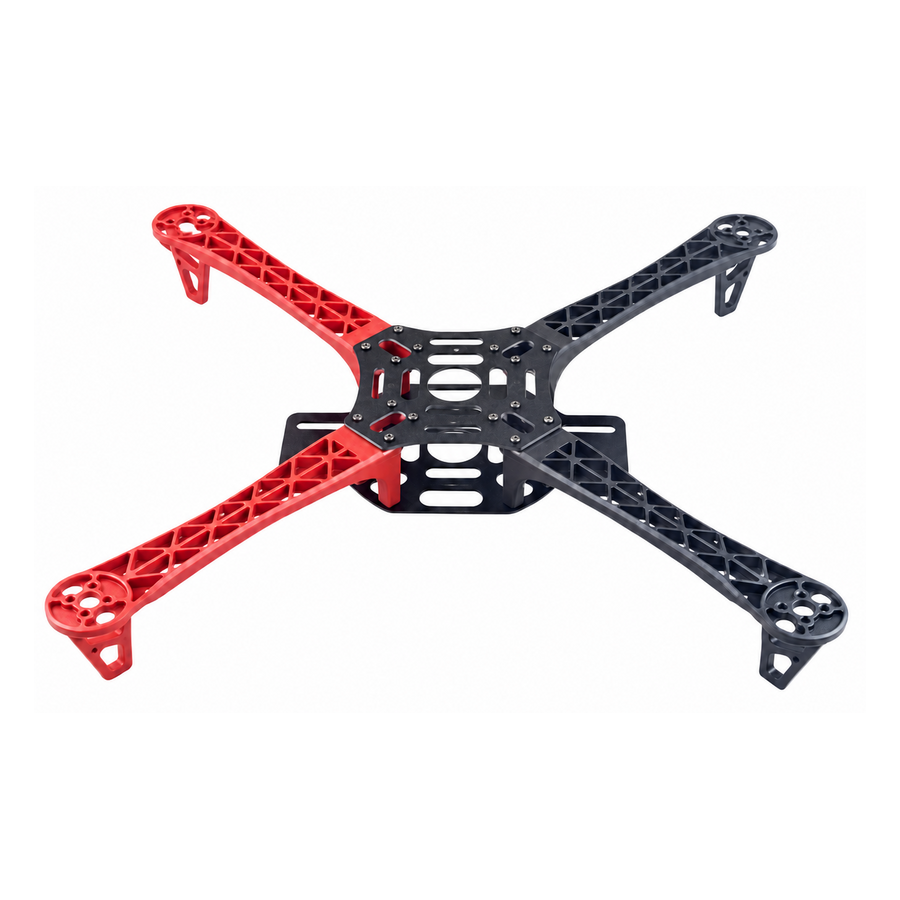
\includegraphics[trim=0 40bp 0 40bp,clip,height=4.0cm]{figures/ch03/f450-frame.png}
	\caption{Bộ khung F450 với hai tấm trung tâm và bốn tay đòn.}
	\label{fig:hardware-f450-frame}
\end{figure}

Bộ khung F450 trong \fref{fig:hardware-f450-frame} gồm hai tấm trung tâm và bốn tay đòn, được bố trí theo cấu hình chữ X~\cite{djiF450Manual}. Động cơ lắp tại đầu các tay đòn; pin, bo điều khiển và các module được bố trí quanh vùng trung tâm.

\begin{table}[H]
	\centering
	\caption{Thông số cơ bản của bộ khung F450.}
	\label{tab:hardware-frame-specifications}
	\begin{tabularx}{\linewidth}{|C{5.0cm}|Y|}
		\hline
		\textbf{Thông số} & \textbf{Giá trị} \\
		\hline
		Loại khung & F450, quadrotor cấu hình chữ X \\
		\hline
		Kết cấu chính & Hai tấm trung tâm và bốn tay đòn \\
		\hline
		Đường chéo hai trục động cơ & 450 mm \\
		\hline
	\end{tabularx}
\end{table}

\clearpage
\subsection{Động cơ không chổi than A2212/10T 1400KV}

Bốn động cơ A2212/10T 1400KV được bố trí tại đầu các tay đòn, mỗi động cơ dẫn động một cánh quạt. Động cơ nhận điện ba pha từ ESC để tạo mômen quay.

\begin{figure}[H]
	\centering
	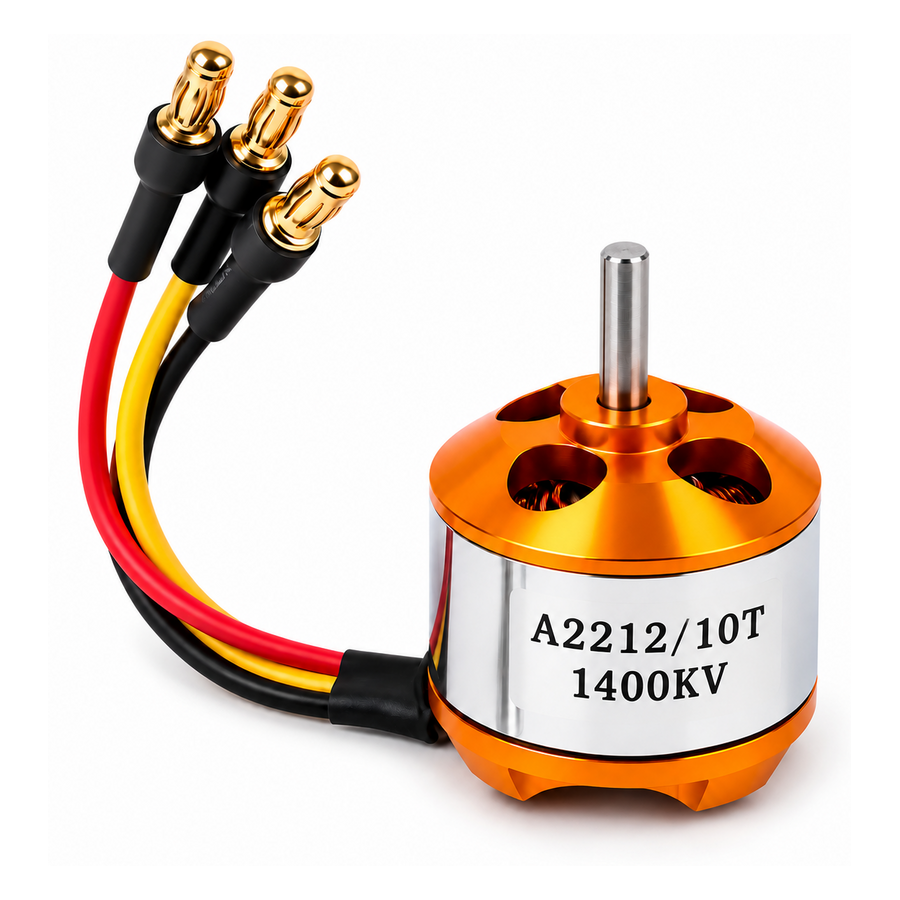
\includegraphics[width=0.43\linewidth]{figures/ch03/a2212-1400kv-motor.png}
	\caption{Động cơ không chổi than A2212/10T 1400KV.}
	\label{fig:hardware-a2212-motor}
\end{figure}

\begin{table}[H]
	\centering
	\caption{Thông số nhận dạng và cấu hình sử dụng động cơ.}
	\label{tab:hardware-motor-specifications}
	\begin{tabularx}{\linewidth}{|C{5.0cm}|Y|}
		\hline
		\textbf{Thông số} & \textbf{Giá trị} \\
		\hline
		Mã ghi trên động cơ & A2212/10T \\
		\hline
		Loại động cơ & Không chổi than, ba pha \\
		\hline
		Hằng số tốc độ $K_V$ & 1400 vòng/phút/V \\
		\hline
		Số lượng & 4 động cơ \\
		\hline
		Cấu hình ghép trong đề tài & Mỗi động cơ ghép một ESC 30 A và một cánh quạt 9 inch \\
		\hline
	\end{tabularx}
\end{table}

Hằng số $K_V$ trong \tref{tab:hardware-motor-specifications} cho biết quan hệ xấp xỉ giữa điện áp cấp và tốc độ quay khi động cơ chạy không tải. Khi lắp cánh quạt, động cơ phải tạo mômen để kéo tải khí động, nên tốc độ quay và dòng điện thay đổi theo cánh quạt và điện áp pin. Vì vậy, khả năng tạo lực đẩy được xét trên cả cụm động cơ--cánh quạt trong điều kiện có tải này.

\clearpage
\subsection{Cánh quạt 9 inch}

Cánh quạt chuyển mômen quay của động cơ thành lực đẩy. Hệ thống sử dụng bốn cánh quạt hai lá, đường kính 9 inch, gồm hai cánh quay thuận chiều kim đồng hồ (CW) và hai cánh quay ngược chiều kim đồng hồ (CCW), xét từ phía trên. Các cánh được lắp phù hợp với chiều quay của từng động cơ để cùng tạo lực đẩy hướng lên.

\begin{figure}[H]
	\centering
	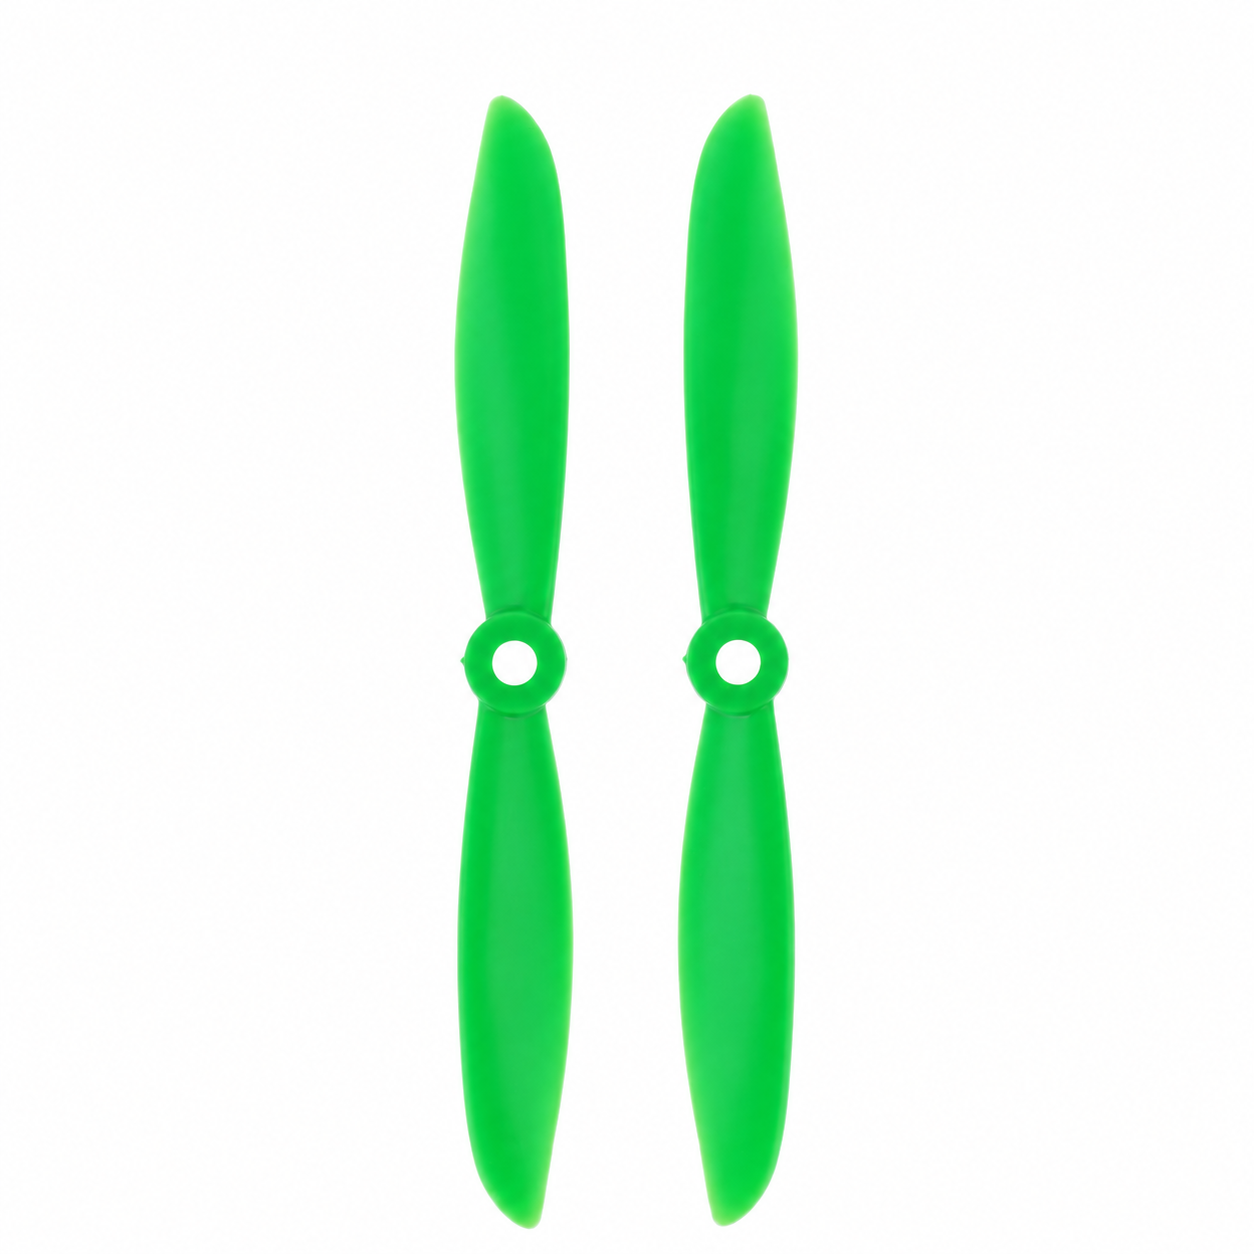
\includegraphics[trim=220bp 0 220bp 0,clip,height=5.2cm]{figures/ch03/propeller-9inch.png}
	\caption{Cặp cánh quạt hai lá minh họa cho cấu hình cánh 9 inch.}
	\label{fig:hardware-propeller}
\end{figure}

\begin{table}[H]
	\centering
	\caption{Thông số cơ bản của cánh quạt trong đề tài.}
	\label{tab:hardware-propeller-specifications}
	\begin{tabularx}{\linewidth}{|C{5.0cm}|Y|}
		\hline
		\textbf{Thông số} & \textbf{Giá trị} \\
		\hline
		Đường kính lựa chọn & 9 inch, tương đương 228,6 mm \\
		\hline
		Số lá trên mỗi cánh quạt & 2 \\
		\hline
		Số lượng & 4 cánh quạt \\
		\hline
		Phân loại chiều quay & 2 CW và 2 CCW, xét từ phía trên \\
		\hline
	\end{tabularx}
\end{table}

Bước cánh hình học biểu thị quãng tiến lý thuyết theo phương trục của cánh quạt trong một vòng quay khi không có trượt~\cite{faaPropellerHandbook}. Bên cạnh đường kính và bước cánh, vật liệu chế tạo ảnh hưởng đến khối lượng, độ bền và độ cứng của cánh quạt. Độ cứng phù hợp giúp hạn chế biến dạng và kiểm soát đáp ứng rung khi cánh quay~\cite{apcPropellerMaterials}. Vì vậy, việc lựa chọn cánh quạt cần xét đồng thời đặc tính khí động và cơ học, bảo đảm phù hợp với động cơ và điều kiện vận hành.

\clearpage
\subsection{Bộ điều tốc ESC 30 A}

Hệ thống sử dụng bốn bộ điều tốc ESC 30 A, mỗi bộ điều khiển một động cơ A2212/10T. ESC nối giữa pin và động cơ, nhận điện một chiều từ pin LiPo 3S và chuyển mạch để cấp điện ba pha cho động cơ.

\begin{figure}[H]
	\centering
	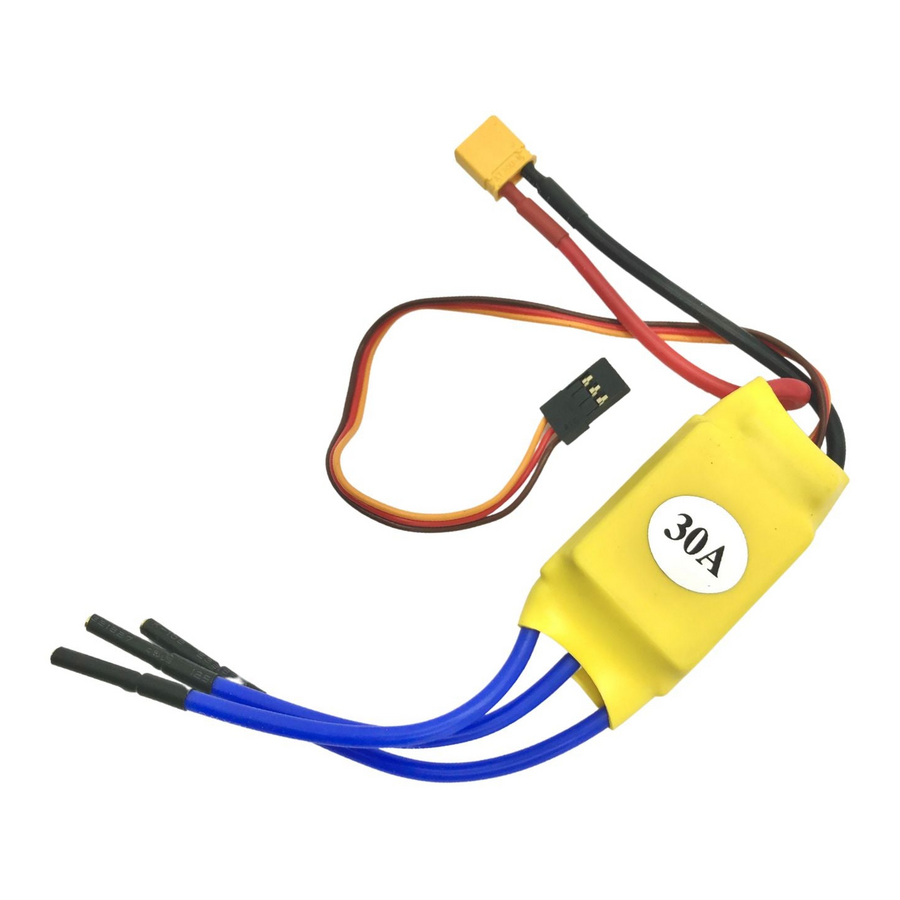
\includegraphics[width=0.43\linewidth]{figures/ch03/esc-30a.png}
	\caption{Bộ điều tốc ESC 30 A.}
	\label{fig:hardware-esc-30a}
\end{figure}

\begin{table}[H]
	\centering
	\caption{Thông số và cấu hình sử dụng ESC.}
	\label{tab:hardware-esc-specifications}
	\begin{tabularx}{\linewidth}{|C{5.0cm}|Y|}
		\hline
		\textbf{Thông số} & \textbf{Giá trị} \\
		\hline
		Dòng điện ESC & 30 A \\
		\hline
		Số lượng & 4 ESC \\
		\hline
		Loại động cơ điều khiển & Động cơ không chổi than ba pha \\
		\hline
		Tín hiệu điều khiển & PWM từ vi điều khiển \\
		\hline
		Nguồn cấp trong đề tài & Pin LiPo 3S \\
		\hline
	\end{tabularx}
\end{table}

STM32 gửi lệnh PWM riêng đến từng ESC để điều chỉnh tốc độ bốn động cơ. Khi tốc độ một động cơ thay đổi, lực đẩy của cánh quạt tương ứng cũng thay đổi. Bằng cách điều chỉnh lực đẩy khác nhau giữa các cụm động cơ--cánh quạt, hệ thống tạo mômen để hiệu chỉnh tư thế quadrotor. ESC đảm nhiệm khâu công suất, chuyển lệnh từ vi điều khiển thành tác động lên động cơ.

Bên cạnh nhánh công suất cấp cho động cơ, mạch BEC (Battery Eliminator Circuit) tích hợp trong ESC2 cung cấp nguồn 5 V cho bo STM32 và bộ thu ELRS.

\clearpage
\subsection{Pin LiPo 3S 5200 mAh}

Pin được sử dụng có cấu hình 3S1P, gồm ba cell mắc nối tiếp trong một nhánh. Bộ pin LiPo có điện áp danh định 11,1 V và dung lượng 5200 mAh, cung cấp năng lượng cho bốn ESC cùng nhánh nguồn điện tử.

\begin{figure}[H]
	\centering
	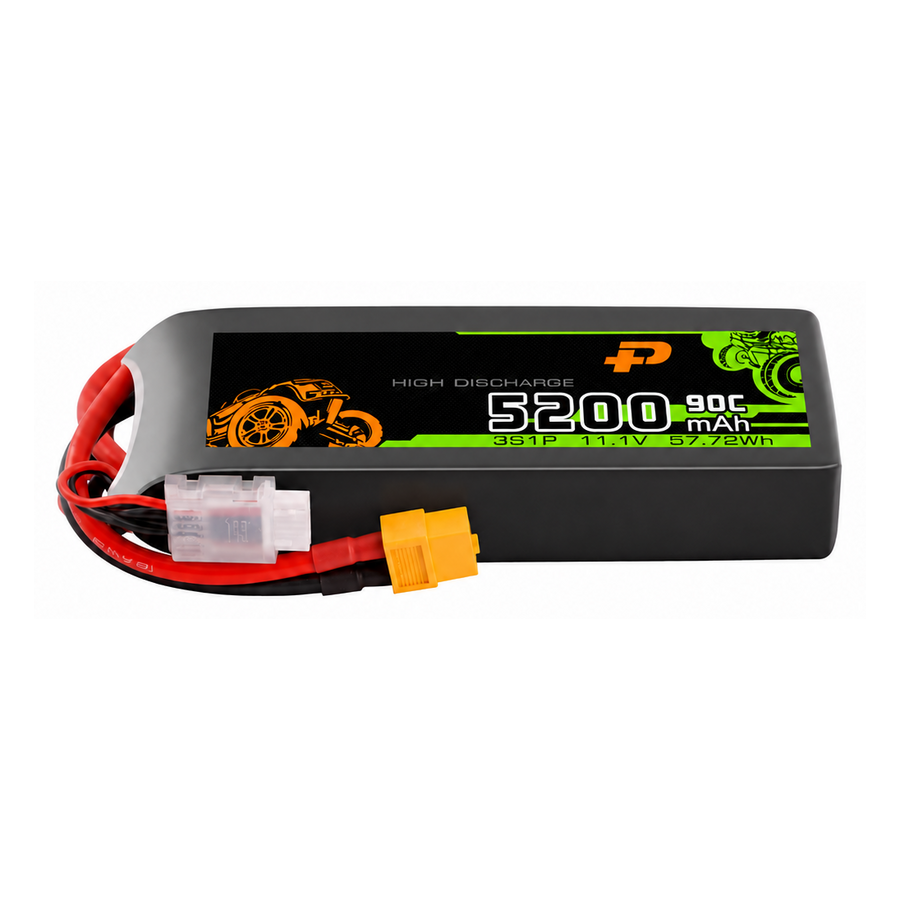
\includegraphics[trim=0 60bp 0 65bp,clip,width=0.60\linewidth]{figures/ch03/lipo-3s-5200mah.png}
	\caption{Pin LiPo 3S1P dung lượng 5200 mAh.}
	\label{fig:hardware-lipo-battery}
\end{figure}

\begin{table}[H]
	\centering
	\caption{Thông số của pin LiPo.}
	\label{tab:hardware-battery-specifications}
	\begin{tabularx}{\linewidth}{|C{5.0cm}|Y|}
		\hline
		\textbf{Thông số} & \textbf{Giá trị} \\
		\hline
		Loại pin & Lithium polymer (LiPo) \\
		\hline
		Cấu hình cell & 3S1P \\
		\hline
		Điện áp danh định & 11,1 V \\
		\hline
		Dung lượng & 5200 mAh (5,2 Ah) \\
		\hline
		Năng lượng danh định & 57,72 Wh \\
		\hline
		Hệ số xả công bố & 90C \\
		\hline
	\end{tabularx}
\end{table}

Khi tăng ga để tăng lực đẩy, dòng điện từ pin cấp cho các động cơ tăng lên. Điện áp giữa hai cực pin cũng thay đổi theo tải và lượng điện còn lại. Dung lượng 5200 mAh cho biết lượng điện tích dự trữ, còn hệ số xả C mô tả khả năng cấp dòng theo dung lượng pin~\cite{grepowLipoCRating}.

\clearpage
\subsection{Lắp ráp cụm cơ khí và nguồn}
\label{subsec:design-mechanical-assembly}

\begin{figure}[H]
	\centering
	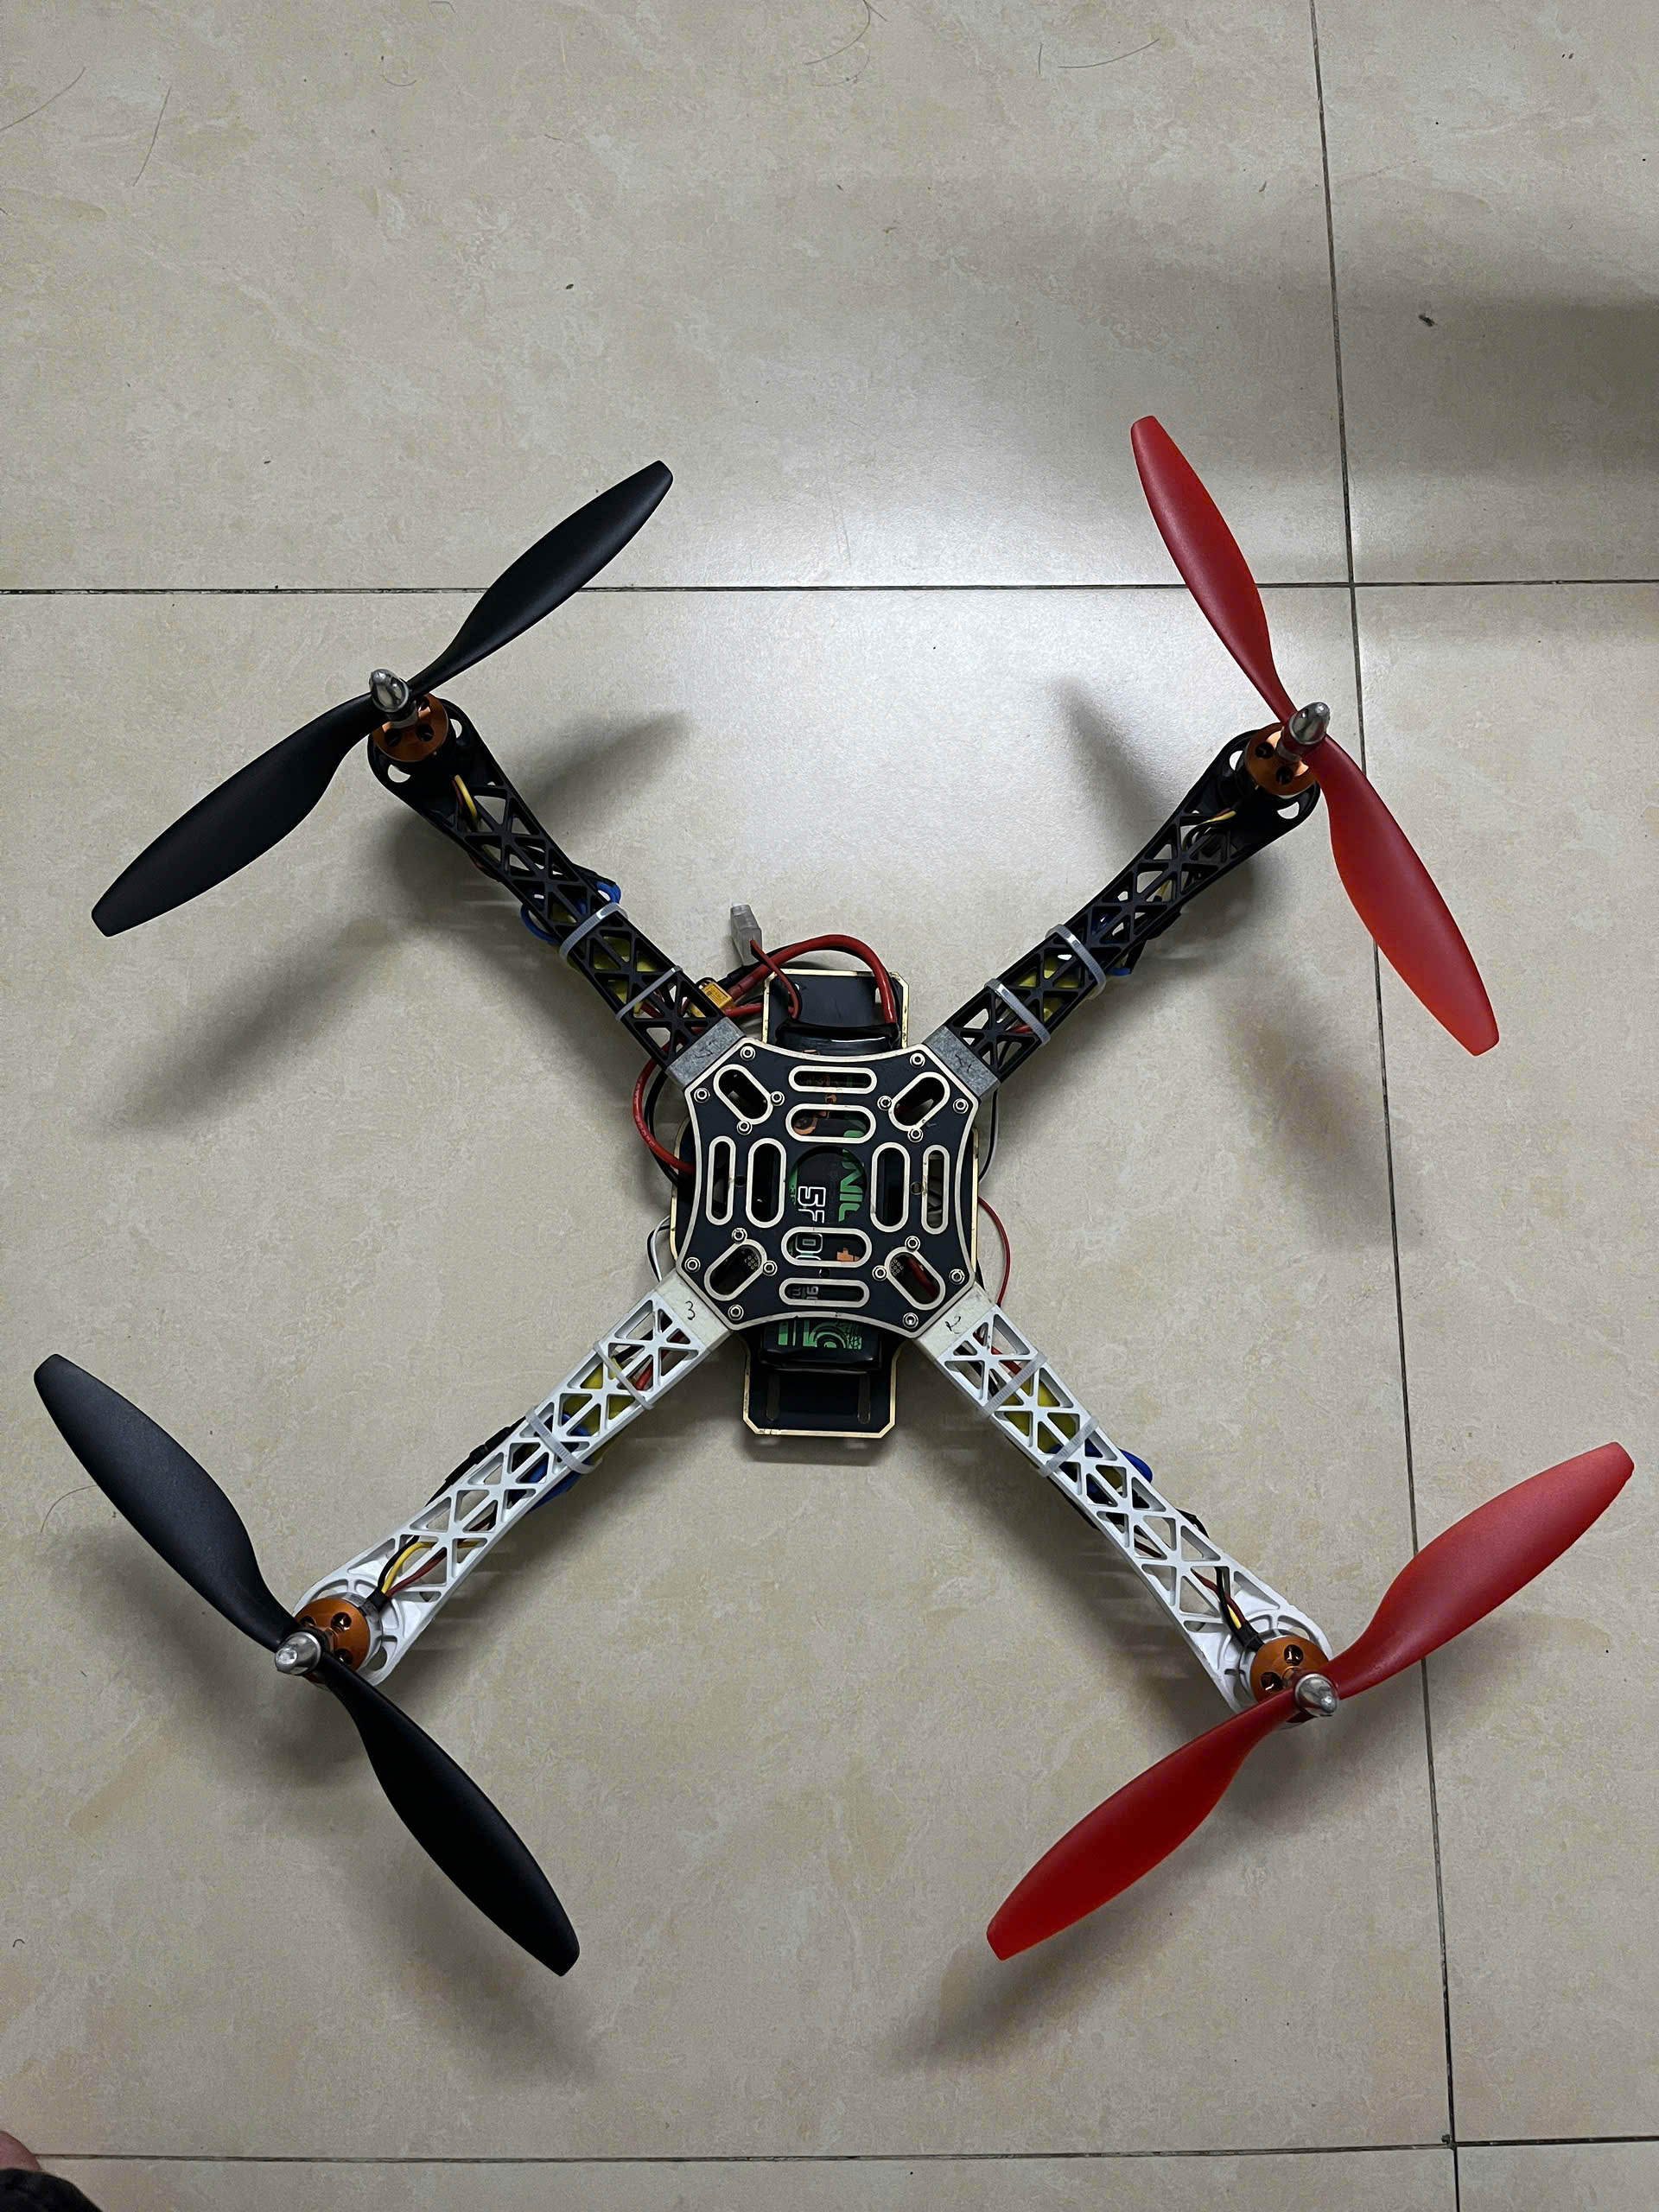
\includegraphics[trim=0 100bp 0 300bp,clip,width=0.90\linewidth,height=12.5cm,keepaspectratio]{figures/ch03/mechanical-power-assembly.jpg}
	\caption{Cụm cơ khí, hệ động lực và nguồn sau khi lắp ráp.}
	\label{fig:design-mechanical-assembly}
\end{figure}

Bốn động cơ được lắp tại đầu các tay đòn của khung F450, đưa các cánh quạt ra ngoài vùng trung tâm thân. Dây nối động cơ được dẫn dọc theo tay đòn và giữ sát khung bằng dây rút. Pin nằm ở vùng giữa thân, bên dưới tấm khung trung tâm; dây nguồn được đưa ra cạnh thân để kết nối với hệ động lực. Các thành phần này tạo thành cụm cơ khí và nguồn trước khi lắp thêm bo điều khiển.
